\documentclass[notes]{beamer}
%\documentclass[notes=only]{beamer}
%\documentclass{beamer}

\usepackage{multicol}
\usepackage{graphicx}
\usepackage{hyperref}
\usepackage{caption}
\usepackage{natbib}
\usepackage{tabularx}
\usepackage{ragged2e}
\usepackage{makecell}
\newcolumntype{C}{>{\Centering\arraybackslash}X}
\usepackage[USenglish]{babel}
\captionsetup[figure]{font=tiny}

\newcommand*{\tabindent}{\hspace{3mm}}

\usepackage{pgfpages}
\setbeameroption{show notes on second screen=left} % 

\graphicspath{ {../../illustrations/} }

\setbeamercolor{author}{fg=white} 
\setbeamercolor{title}{fg=white} 
\setbeamercolor{date}{fg=white} 
\setbeamercolor{institute}{fg=white} 

\logo{
\includegraphics[height=1.5cm]{ivey.jpg}}
\setbeamertemplate{footline}[frame number]

\title{Proposal Defense}
\subtitle{Greenwashing and Learning in the Pipeline Industry}
\author{Julian Barg}
\date{September 22, 2020}
\institute[Inst.]{Ivey Business School}

\definecolor{ivey-green}{HTML}{034638}
\definecolor{ivey-purple}{HTML}{582C83}

\AtBeginSection[]
{
	\begin{frame}
		\frametitle{Table of Contents}
		\tableofcontents[currentsection]
	\end{frame}
}


\begin{document}
	{\setbeamercolor{background canvas}{bg=ivey-purple}
		\frame{\titlepage}  
	}

	\begin{frame}{Outline of talk}
		\tableofcontents
		\begin{itemize}
			\item Refresher (very brief)
			\item Framework
			\item Phenomenon
			\item Framing/Theories
			\item Papers
			\item Timelines
		\end{itemize}
		\note{I feel a little bit like I am at a wedding where there are two separate families that you need to bridge. So I am going to do that by spoon-feeding you a few select insights on the two literatures. I very much designed this presentation as a series of questions--which I may forget if I get carried away.}
	\end{frame}

	\section{Introduction}

\begin{singlespace} 
	\begin{quote}
		"[T]here is perhaps an over-emphasis of technology in [Leak Detection Systems]. A recurring theme is that of false alarms. The implication is that [a Leak Detection System] is expected to perform as an elementary industrial automation alarm, with an on/off state and six-sigma reliability. Any alarm that does not correspond to an actual leak is, with this thinking, an indicator of a failure of the LDS system. Instead, multiple technical studies confirm that far more thought is required in dealing with leak alarms" -- \citet[p. 2-3]{Shaw2012}.
	\end{quote}
\end{singlespace}

How does an industry get stuck with a never-ending series of pollution events? It is the conventional view of organizational learning that performance measures, after initially exhibiting fast improvements, will settle at at a certain level \citep{Argote2013-1}. In other words, learning levels off. The \textit{organizational knowledge} view--the dominant stream of the learning literature--suggests that organizations accumulate knowledge which is held by individuals, in routines, or in transactive memory systems \citep{Bingham2011, Argote2011}. New knowledge is added to an existing "stock", presumably until there is no more new insights to be added. Disclosure of the outcomes of this learning process then is a subsequent, separate step--the organization makes a strategic decision as to which outcomes to share with stakeholders. To withhold negative information on environmental performance in this step would constitute greenwashing \citep{Lyon2011}.

An alternative view suggests that organizations can break out of existing trajectories and escape their constraints in learning--but that to do so requires a considerable rethinking of existing paradigms \citep{March2010}. For instance, an organization can reimagine how it measures performance \citep{Argyris1978}. This is consistent with the \textit{organizational routines} view, which holds that organizations develop not knowledge but patterns of action in stable environments \citep{Bingham2011}. The organizational routines view also postulates that in the absence of significant interventions, intricate but ultimately obsolete systems develop, for instance ones that rely on outdated technologies \citep{March1991}. With sufficient complexity, these systems can generate a never-ending stream of unexpected interactions and externalities, which then become relevant for sustainability research when the organization or industry has a catastrophic potential \citep{Perrow1984, Beck1992}. One would hope for stakeholders to be able to identify the pattern of unexpected interactions and externalities, but under an inadequate environmental regime the organization or industry can escape scrutiny through greenwashing \citep{Lyon2015}.

The inconsistent predictions of the two views, and their implications for persistent environmental pollution raises two questions. (1) \textit{How does the convergence of performance measures take place?} When the convergence has taken place in an organization or industry, do we see evidence for either the organizational knowledge or the organizational routines view? The organizational knowledge view suggests that once performance has converged, either no new knowledge is gained, or knowledge disappears at the same rate as it is produced \citep{Argote2013-3}. The organizational routines view makes no such prediction, instead, if that view was accurate we would see increasingly intricate routines with ultimately have little impact on performance. 

An obvious extension to the first question is a look at possibilities for organizations to break out of a state of convergence. The \textit{organizational routines} literature holds that organizations can break out of a state of convergence through what the \textit{organizational routines} literature calls either double-loop learning \citep{Argyris1978} or high-intellect learning \citep{March2010}. Two overlooked attributes of knowledge, \textit{validity} and \textit{reliability} could mend the split between the two streams of the organizational learning literature. \textit{Validity} describes whether knowledge does allow an organization to better understand, predict, and control problems, such as technological limitations or bottlenecks. \textit{Reliability} describes the degree to which member of the organization have command of the knowledge \citep{Rerup2020}. Validity and reliability allow for a critical view on the first question, and whether that state of convergence is inevitable.

(2) The state of convergence should be fairly obvious to stakeholders when environmental pollution is involved. The second research question addresses the difficulties that continuous environmental pollution would be expected to entail. \textit{How does an organization manage--or greenwash--its convergence to a state of constant pollution?} If the state of convergence is obvious for observers, one would expect calls for substantive change to be quite loud. But the pipeline industry has maintained the status quo for twenty years, which presumably requires an effort to maintain the status quo rather than just an absence of efforts to break out of the state of convergence.

%Learning is more complex than the existing view would suggest--organizations can leave an existing trajectory, but requires a considerable rethinking of existing paradigms \citep{Argyris1978, March2010, March1991}. An explanation for the divergence within the existing literature are two overlooked attributes of knowledge: validity and reliability \citep{Rerup2020}. The disclosure of information on environmental performance is closely related to the generation of knowledge and beliefs. The existing literature considers greenwashing to be a strategizing process that occurs when environmental outcomes are already determined \citep{Delmas2011}. Existing research on intra-industrial processes however suggest that information disclosure and the generation of new knowledge are closely related \citep{Maguire2009}. This dissertation deciphers the processes of knowledge creation, convergence of environmental performance, and greenwashing through two research questions. (1) \textit{How does an organization that effectively learns from failures also stagnate?} And (2) \textit{how does an industry greenwash its stagnatioinn in environmental performance?}

To answer the research questions, this dissertation employs data on the US pipeline industry. The pipeline industry offers an advantage over other industries with regard to studying environmental impacts, learning, and greenwashing, in that the industry's environmental pollution very much takes place in the public. Unlike other industries, pipeline spills do not occur inside private plants, locked away from the public eye. Pipeline spills usually occur on public land that the pipeline operator has only acquired the right-of-way of. Pipeline spills also receive a lot of attention from the press, government agencies, and environmental grassroot organizations. These actors pay particular attention to large pipeline spills, which make up for a majority of annual spill volume. Finally, the scrutiny of oil spills also ensures that the reported data is more accurate. Government-employed emergency responders are on site alongside the company employees and can ensure a more accurate reporting of pollution data than is the case for routine environmental emissions.

Quantitative data from 2004-2019 allows us to observe learning and greenwashing in the pipeline industry. For this period of time, data is available from the Pipeline and Hazardous Materials Safety Administration (PHMSA) on how much oil each American operator transported over what distance every year. PHMSA also provides a dataset that contains data on each individual pipeline spill that occurred over that period of time.\footnote{See \url{https://www.phmsa.dot.gov/data-and-statistics/pipeline/source-data}, accessed 2020-08-30}. Data on the spills includes a narrative, how much oil was spilled and recovered, and what other impacts (e.g., injuries or deaths) occurred. Over the 16 years of the observation period, 6,147 pipeline spills were recorded, including 2,246 that the PHMSA classified as significant based on either a spill volume of over 50 barrels, more than \$50k in damages, or a casualty, injury, fire or explosion. Whereas crude oil pipelines period showed a significant improvement in pipeline safety over the observation period, the standardized spill volume of refined petroleum pipelines stayed as an almost constant rate of about 15bbl per billion barrel-miles transported (see Figure 1). 

Qualitative data provides an understanding of the mechanisms of learning in the pipeline industry. That constant spill rate for refined petroleum pipelines is surprising, given the significant technological advancements in the areas of inline inspection tools, leak detection, and SCADA systems which allow for the remote supervision and control of pipelines. A repository on the largest or otherwise significant pipeline spills by the National Transportation Safety Board (NTSB) provides an in-depth understanding of accident causes. Since 1969, NTSB has authored 142 accident reports and briefs.\footnote{See \url{https://www.ntsb.gov/investigations/AccidentReports/Pages/pipeline.aspx}, accessed 2020-08-30}. For this dissertation I select the 10 most recent full accident reports. As a robustness check, I also select the 15 most significant accidents according to spill volume, net loss, number of injuries and fatalities, and property damage (top 3 per category), and collect independent archival data on these spills. As of 2020, little empirical research exists on the pipeline industry. \citet{Park2019} uses the PHMSA dataset to study how reputation affects relationships with exchange partners. \citet{Zakikhani2020} review the research into pipeline failures in the area of engineering, which has largely ignored organizational factors. 

Finally, this dissertation uses text and network data for track greenwashing in the pipeline industry. Headquarter locations and board memberships (BoardEx) uncover connections between pipeline operators. Documents by the American Petroleum Institute (API) and the Association of Oil Pipe Lines (AOPL) reveal developments of the industry level. In addition, this research uses annual reports and safety reports to determine the strategies pursued by individual operators. Natural Language Processing (NLP)--specifically, topic modeling--reveals trends and show their diffusion through the pipeline industry. Finally, we can compare trends with the topics that emerge from the narratives on pipeline spill to distinguish substantive and non-substantive trends.

The context of pipeline spills is suitable for both questions on learning and greenwashing. Pipeline spills, such as other failures, are catalysts for learning \citep{March1991}. In the pipeline industry, learning has high visibility after large pipeline spills take place. We can observe the learning process independent of its outcomes better than in other contexts. Oil spills also bring pipeline operators under high scrutiny. As a result, pipeline safety often enters the public debate. The American Petroleum Institute (API) and the Association of Oil Pipe Lines (AOPL) discuss pipeline safety and their communication strategy in a semi-public fashion. Documents by operators on pipeline safety are also public and widely available. When greenwashing takes place in the pipeline industry, it is a public affair. It is thus easier to obtain data on learning and greenwashing for this industry, compared to most other industries, which operate far less on public lands.

{\noindent}\dotfill

	\centerline{Insert Figure 1 about here}

{\noindent}\dotfill

\begin{figure}
	\caption{Pipeline safety improvements at the industry level}
	\centerline{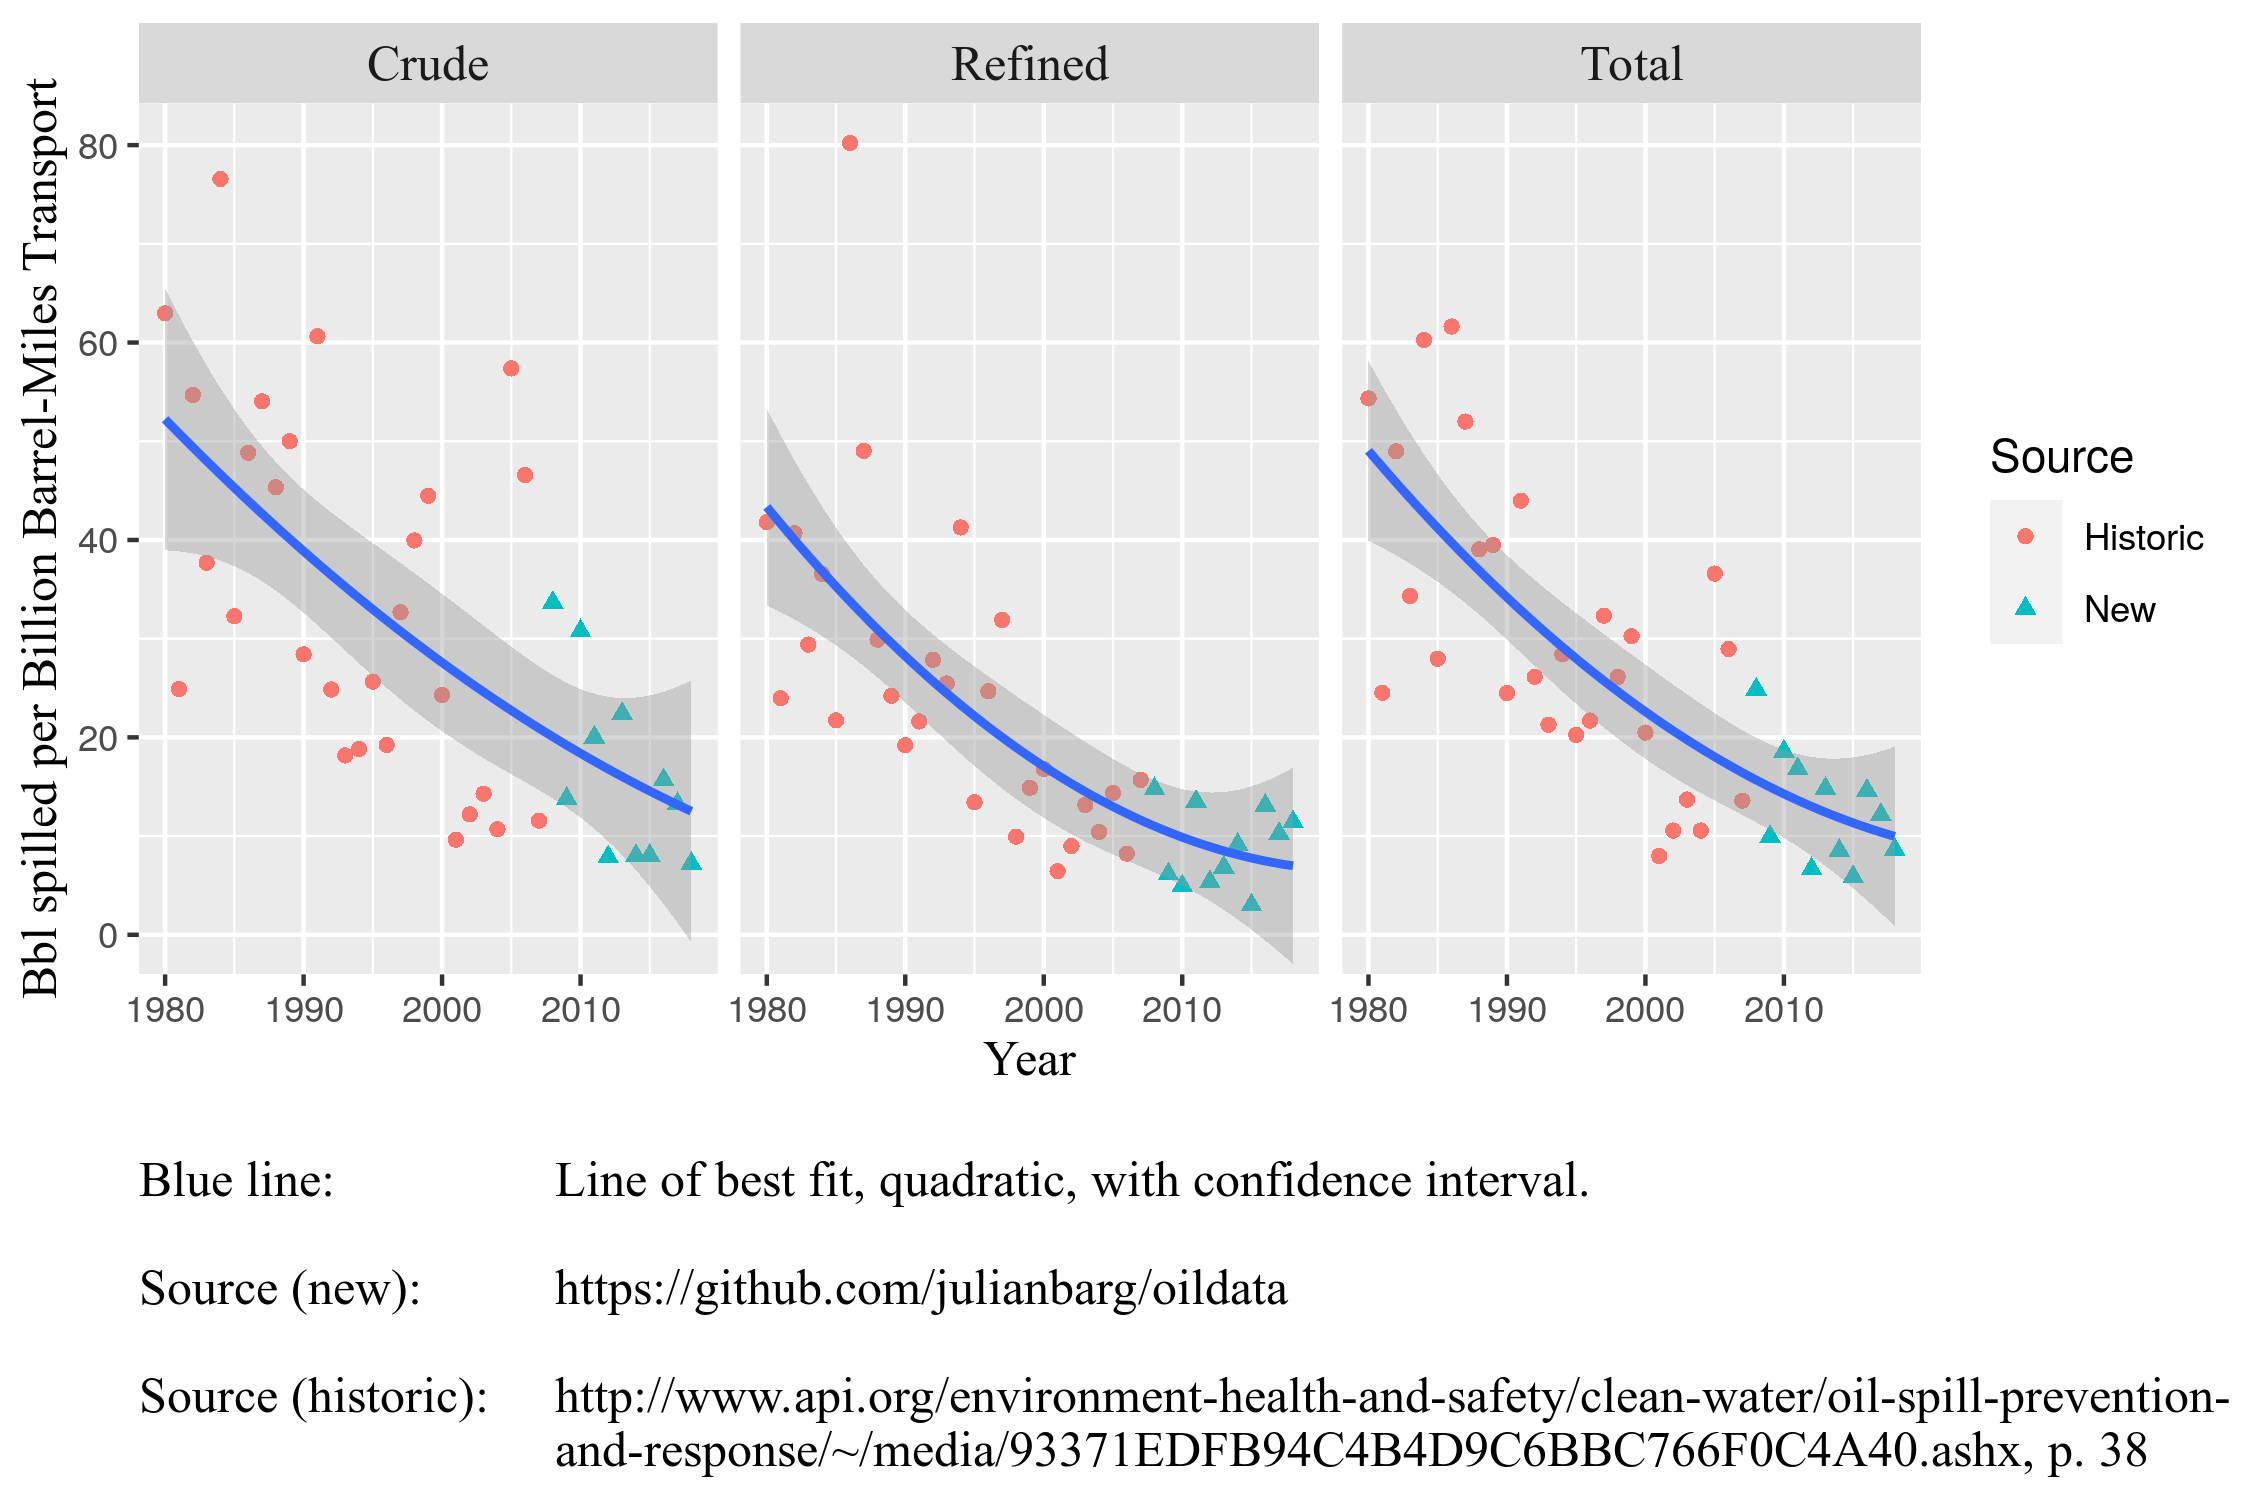
\includegraphics{../illustrations/population_learning_4.png}}
\end{figure}

Some of the findings of this dissertation might not be fully generalizable. Pipeline systems, with their manifold interactions and catastrophic potential are a great example of the complex systems and externalities discussed by \citet{Perrow1984} and citet{Beck1992}. The challenges associated with growing complexity may not be present in all other contexts. In particular, uncoupled production methods can allow for much reduced interactive potential. In these contexts, convergence of performance measures and greenwashing might take on a different shape. The complexity of pipeline systems stems from the interaction of mechanics, physics (fluid dynamics are notoriously complicated are of physics), and a complicated command structure. The diverse geography and many jurisdictions of the US also add to the complexity. In addition, there is an economic incentive to run pipeline infrastructure at a very high utilization rate and throughput, e.g., by frequently changing the commodity to be transported according to demand.\footnote{Although pipelines are generally optimized for transporting specific commodities, in principle any pipeline can transport almost any commodity when demand or supply changes.} Altogether, the complexity and interactions are not far off from what \citet{Perrow1984} observed for nuclear power plants. Many other industries constitute complex systems because of their elaborate supply chain structures, a future avenue of research would thus be whether these complex supply chains bring about the same limits to learning.

I make four contributions with this research. (1) This dissertation introduces a context where organizational learning has "bottomed out" and analyzes how learning plays out under these circumstances. The context allows us to study learning despite the absence of aggregate, quantitative improvements in performance measures because (a) we can observe the process of learning independent from the outcome in qualitative data, and (b) rich data, including textual descriptions, is available on the object of learning--individual pipeline spills. This rich data allows us to distinguish a "dynamic" state where performance measures are constant because learning and emerging challenges cancel each other out from a hypothetical "state of equilibrium" where there is no new knowledge to be obtained. Thus, this dissertation brings to the fore a state that large swaths of the learning literature have taken for granted: the "end of learning" period where performance measures make it appear as if the organization has come to a standstill. At least for this case of a complex system with catastrophic 

(2) This dissertation also makes a contribution to the discourse regarding environmental sustainability and technology. The sustainability research community is split as to the role of technology for sustainability. Some work leans more toward a technocentric view with little to no consideration of social systems, for instance in research on low-carbon electricity \citep[e.g.,][]{Greenblatt2017}. Other authors emphasize the need for changes to the political and economic system in order reduce damages to the planet, such as the degrowth discourse \citep{Kallis2018}. With regard to that debate, the findings of this research highlight the role that system complexity and unexpected externalities play for continued pollution. The pipeline industry provides a very vivid example of the limits to depolluting existing technology. Further, the greenwashing in the pipeline industry that this research surfaces should act as a cautionary tale on the role and purpose of technology in communication.

(3) This dissertation moves forward theory on learning by highlighting the considerable effort necessary to leave an existing trajectory. New knowledge needs to be created that is both valid and reliable, which requires for an organization or industry to collectively question preexisting fundamental assumptions. Applied to pipeline spills, this would imply that if society was to collectively decide that oil spills at the current level are not acceptable, then we should not rely on the industry to develop technology and make changes in the current fashion. A more fundamental rethinking of the (physical and political) system of energy delivery would be necessary.

(4) The empirical research on greenwashing highlights the potentially malevolent role that industry level organizations can play, and that technology should be taken with reservation. Actors in the pipeline industry are aware of the possibility to created a better image by creating an association between pipelines and high-tech, even in the absence of better safety performance. These actors may also be aware that is almost impossible for laymen to rebut the validity of technology that is built on decades of engineering research, and that hence the industry can safely entrench itself in this modern realm.

%The empirical sections of this dissertation use data from the US pipeline industry. Compared to other industries, both environmental pollution events and the subsequent learning process play out in a very public fashion in the pipeline industry. Large spills, which make up for a big share of the overall spill volume, are often discovered by members of the public, covered by the press, and investigated by independent government agencies. The context offers two advantages over existing empirical research. First, in the pipeline industry we can disentangle learning and the outcomes thereof. Empirical research on organizational learning commonly has to rely on improvements in performance variables to gauge learning \citep{Argote2011}. As in the context of the pipeline industry learning can be observed directly, the risk of an outcome bias is reduced \citep{Dillon2008}. The context also allows us to disentangle effective learning and rhetorics or greenwashing. In the pipeline industry, it is possible to determine when new technology and other measures are a response to existing problems, and when they are ineffective or even misleading talking points that serve to greenwash. The latter, in this specific context, is tied to industry level organizations such as the American Petroleum Institute (API) or the Association of Oil Pipe Lines (AOPL).

%This dissertation addresses two questions. (1) Can organizations that effectively learns from failures \citep{March1991} also stagnate? And (2) how does does an industry greenwash \citep{Lyon2015} this stagnation? Organization learning is observed to, after initially quick progress, converge to a certain value \citep{Argote2013-1}. In this process, organizations develop advanced, complex systems. \citet{Beck1992} and \citet{Perrow1984} suggest that unexpected interactions and externalities are intrinsic limitations of these systems. Only considerable rethinking of existing paradigms allows organizations to break out of the dead end that these complex systems can become \citep{Argyris1978, March2010, March1991}. The key to this breakout is validity and reliability of knowledge \citep{Rerup2020}. \citet{Lyon2011} suggest that instead of addressing externalities in the environmental realm, organizations may prefer to greenwash \citep{Lyon2011}. Trade associations are known to play a role in processes such as greenwashing when it occurs on a larger scale \citep{Maguire2009}.

%Between in-line inspection tools, leak detection technology, and SCADA systems that allow for the remote supervision and control of pipelines, it seems as if the pipeline industry has a technological solution to every problem thrown at it. \textit{Then why has the industry not improved its environmental performance in twenty years?} Further, if pipeline spills in the year 2020 are still common, this raises a follow-up question: \textit{How do pipeline operators regularly convince their stakeholders and the regulator that pipelines are safe}, and that they should be allowed to expand their physical footprint.


%Organizational forgetting ultimately is a routines view.
	\frame{
	\insertsection{Theories}
}

\begin{frame}
	\frametitle{Greenwashing}
	\begin{enumerate}
		\item \citet{Delmas2011}
		\item \citet{Lyon2011}
		\item \citet{Lyon2015}
		\item \citet{Marquis2016}
		\item \citet{Kim2015}
	\end{enumerate}

	\vspace{0.1cm}
	\hrule
	\vspace{0.1cm}
	\small
	Definitions: "any communication that misleads people into adopting overly positive beliefs about an organization’s environmental performance, practices, or products" \citep[p. 226]{Lyon2015}.

	\note{
		\tiny
		\begin{enumerate}
			\item \citet{Delmas2011}--explaining that greenwashing can be cheaper than action. Motivations for greenwashing range from internal communication problems to problematic incentive structures.
			\item \citet{Lyon2011}--economic perspective on greenwashing. Economic rational. Predicting that greenwashing more likely when good environmental performance moderately surprising. Since if its not surprising, firm gains no benefit for having positive performance. And similarly, if it is not surprising, firms gain little from disclosing negative performance. Applicable to my empirical context--it \textit{is} surprising if pipeline operators have persuasive evidence that they are save and clean. And what we see in the empirical context is exactly partial disclosure.
			\item \citet{Lyon2015}--differentiating different kinds of greenwashing. Distinguishing between decoupling and calculated economic greenwashing, and marketing. Providing definition.
			\item \citet{Marquis2016} Role model for large scale greenwashing study. Constructing a variable that captures how much of an organization's environmental disclosure is composed of metrics that actually matter, and how much of it consists of irrelevant metrics. Nice, large scale study, good statistical power \textit{but} the DV is misconstructed.
			\item \citet{Kim2015}--alluding to the fact that a lot more of the communication organizations do is political. Introduces brownwashing: deliberate obfuscation of good environmental performance as not to raise expectations or in case shareholders think anything green is expensive. Overall, gives off the impression that we can take environmental information far less at face value than we thought.
		\end{enumerate}
	}
\end{frame}

\begin{frame}
	\frametitle{Organizational learning}
	\begin{enumerate}
		\item \citet{March1963}
		\item \citet{Argyris1978}
		\item \citet{March1991}
		\item \citet{Argote2013}
		\item \citet{March2010}
	\end{enumerate}

	\note{
		\tiny
	\begin{enumerate}
		\item \citet{March1963} Mostly talking about learning in terms of routine adjustments, but also e.g., of attention and search rules. Important element: emphasizing the political nature of how priorities are set and what is being learned--reliability!
		\item \citet{Argyris1978} Double-loop learning. Learning is more complex than adjustments of inputs and outputs. At some point, fundamental assumptions need to be questioned in order to make an impact--there are a lot of iron tenets in the pipeline industry or fossil fuel in general that are not being touched. Gives the example of changing performance measures that are used to track progress. Maybe pipelines should stop their ridiculous 99.9999\% success rate--now they are focusing on zero accidents--good.
		\item \citet{March1991} I guess Mark may not agree that this should be here as an important paper. But--does a good job of showing that going deeper and deeper on one technology does not hold as much promise as regularly straying far away--exploration!
		\item \citet{Argote2013} Mostly literature review and representative of the knowledge-based view. Which I find problematic, because it fails to recognized the distributed nature of "knowing" in organizations and the interests that clash--politics!
		\item \citet{March2010} Differentiating high-intellect and low-intellect learning. But more importantly, introducing (very briefly) validity and reliability as attributes of knowledge. Knowledge is reliable if it is shared among members of an organization/population. It is valid if it actually helps to bring about its goal/make a difference.
	\end{enumerate}
	}
\end{frame}
	\begin{frame}
	
	\tiny
	\begin{tabularx}{\textwidth}{l l l p{1.5cm}}
							&Paper 1 					&Paper 2 						&Paper 3 \\
							&Greenwashing 				&Learning in the industry		&Learning theory development \\
		\hline\hline
		Data (primary)		&\textbf{Text data}
										 				&\textbf{Spill data}			& --\\
							&Organization's safety strategy
														&Annual spill volume			& \\				
		Data (auxiliary)	&$\bullet$ Network data		&$\bullet$ Spill description	& --\\
							&$\bullet$ Spill data		& 								& \\
							&\hspace{\parindent} (To assess change to safety)
														&								& \\
		Data sources		&$\bullet$Annual reports	&$\bullet$PHMSA datasets		& --\\
							&$\bullet$BoardEx			&$\bullet$LexisNexis			& \\
							&$\bullet$PHMSA datasets	&$\bullet$Compustat				& \\
							&$\bullet$LexisNexis		&								& \\
							&$\bullet$Compustat			&								& \\
		DV					&Peer group/industry language
														&Pipeline spills				& --\\
		IV					&Focal firm policy			&Same-type spills				& --\\
		Methods				&Panel regression			&Diff-in-diff/moderation		&Theory paper \\
		Moderation			&--							&Emergence of other failure sources
																						& --\\
		
		Auxiliary analysis	&Discourse analysis			&Qualitative analysis of spills & --\\
	\end{tabularx}

	\vspace{0.1cm}
	\hrule
	\vspace{0.1cm}
	
	\textbf{Explanations}	
		
	\textit{Greenwashing paper}: Focal company communication is influenced by technology that is promoted peers and the industry over safety needs.
	
	\textit{Organizational learning}: Pipeline spills lead to improvements in specific areas. But new failure sources emerge to make up for it.
\end{frame}
	\begin{frame}
	\frametitle{Timeline}
	\framesubtitle{Chapter 1}
	\tiny
	\begin{tabular}{ l l }
		Chapter 1 & \\
		Data collection	& \\
		\tabindent Sample creation (PHMSA \& LexisNexis)	& 5 days\\
		\tabindent Data merging (Compustat)					& 4 days\\
		Modeling											& \\
		\tabindent Initial model							& 4 days\\
		\tabindent Feedback \& iterate \#1					& 5 days\\
		\tabindent Feedback \& iterate \#2					& 5 days\\
		Writing												& \\
		\tabindent Readings									& 4 days\\
		\tabindent Introduction								& 3 days\\
		\tabindent Lit review \& hypothesis development		& 4 days\\
		\tabindent Methods \& results						& 5 days\\
		\tabindent Discussion								& 4 days\\
		Feedback \& iterating								& \\
		\tabindent Iteration \#1 -- writing \& style		& 3 days\\
		\tabindent Iteration \#2 -- content					& 5 days\\
		\tabindent Iteration \#3 -- content					& 5 days\\
		\tabindent Iteration \#4 -- writing \& style		& 2 days\\
		\hline
		Approx. 60 days (+ 10 days) = approx. Dec 31--without qualitative data!
	\end{tabular}
	\note{Good news--I finished a whole lot of backend work for PHMSA data over the last 2 weeks.}
\end{frame}

\begin{frame}
	\frametitle{Timeline}
	\framesubtitle{Chapter 2}
	\tiny
	\begin{tabular}{ l l }
		Chapter 2 & \\
		Data collection	& \\
		\tabindent Sample creation (PHMSA \& LexisNexis)	& 5 days\\
		\tabindent Data collection--Annual Reports			& 7 days\\
		\tabindent Data collection--industry level text		& 2 days\\
		\tabindent Text processing							& 5 days\\
		\tabindent Data merging								& 4 days\\
		Modeling											& \\
		\tabindent Initial model							& 5 days\\
		\tabindent Feedback process?						& ?\\
		Writing												& \\
		\tabindent Readings									& 2 days\\
		\tabindent Introduction								& 3 days\\
		\tabindent Lit review \& hypothesis development		& 4 days\\
		\tabindent Methods \& results						& 6 days\\
		\tabindent Discussion								& 4 days\\
		Feedback \& iterating								& \\
		\tabindent Iteration \#1 -- writing \& style		& 3 days\\
		\tabindent Iteration \#2 -- content					& 5 days\\
		\tabindent Iteration \#3 -- content					& 5 days\\
		\tabindent Iteration \#4 -- writing \& style		& 2 days\\
		\hline
		Approx. 60 days + 10 days + ? feedback process = some time in Jan--without discourse analysis!
	\end{tabular}
	\note{Notice the question mark on feedback for NLP/modeling here.}
\end{frame}

\begin{frame}
	\frametitle{Timeline}
	\framesubtitle{Chapter 3}
	\tiny
	\begin{tabular}{ l l }
		Chapter 3 & \\
		Preparation													& \\
		\tabindent Organizing literature							& 5 days\\
		\tabindent Graphical model or structure						& 1 day	\\
		\tabindent Wait												& ?	\\
		\tabindent Feedback/discussion								& 1 day \\
		\tabindent Wait												& ? \\
		\tabindent Iteration										& 1 day \\
		Writing														& \\
		\tabindent Introduction										& 4 days\\
		\tabindent Lit review										& 6 days\\
		\tabindent Theory											& 5 days\\
		\tabindent Discussion										& 5 days\\
		\tabindent Conclusion										& 3 days\\	
		Feedback													& \\	
		\tabindent Iteration \#1 -- writing \& style				& 3 days\\
		\tabindent Wait												& \\
		\tabindent Iteration \#2 -- content							& 4 days\\
		\tabindent Wait												& \\
		\tabindent Iteration \#3 -- content							& 3 days\\
		\tabindent Iteration \#4 -- writing \& style				& 2 days\\
		\hline
		Approx. 50 days + 8 days + ?? wait = late Dec/early Jan?
	\end{tabular}
	\note{Notice the wait here after many steps.}
\end{frame}

\begin{frame}
	\frametitle{Timeline}
	\framesubtitle{Overview}
	\begin{enumerate}
		\item \textbf{Chapter 1}: 60 days
		\item \textbf{Chapter 2}: 60+ days
		\item \textbf{Chapter 3}: 50++ days		
	\end{enumerate}
\end{frame}
		\section{Conclusion}
	\begin{itemize}
		\item Reliability and validity: could look into that for answers/solutions.
		\item What areas of \citet{George2016} are not covered? I will pick those off in future research and could set that up here.
		\item Limitation: assuming that spills encompassing.
	\end{itemize}
	
	\begin{frame}[allowframebreaks]
		\tiny
		\bibliography{../../bibliography}
		\bibliographystyle{apalike}
	\end{frame}
\end{document}